\documentclass{article}
\usepackage[final]{neurips_2025}
\usepackage{lineno}
\linenumbers

\usepackage[utf8]{inputenc}
\usepackage[T1]{fontenc}
\usepackage{hyperref}
\usepackage{url}
\usepackage{booktabs}
\usepackage{amsfonts}
\usepackage{amsmath}
\usepackage{nicefrac}
\usepackage{microtype}
\usepackage{xcolor}
\usepackage{graphicx}

\title{Reproducing Batch Normalization: Effects on Optimization, Stability, and Learning Rate Sensitivity}

\author{
  Hetang Mehta \quad Nathan Krosel \quad Maanas Saxena \quad Nathan Wong \\
  University of Alberta
}

\begin{document}

\maketitle

\begin{abstract}
Batch Normalization (BN) improves deep neural network training by stabilizing intermediate layer
distributions. In this work, we reproduce key experimental findings from Ioffe \& Szegedy (2015)
using simplified settings. We replicate (1) accelerated convergence in a sigmoid-based fully
connected network on MNIST, and (2) improved stability at high learning rates in CNNs on
CIFAR-10. Our results show that BN improves final accuracy by up to 24 percentage points and
prevents training failure at high learning rates, confirming the core qualitative claims of the
original paper. We additionally validate these findings through ablation studies varying hidden
layer width and optimizer type.
\end{abstract}


%% =============================================================================
\section{Summary of the Paper}
%% =============================================================================

Ioffe and Szegedy~\cite{ioffe2015batch} identify a fundamental challenge in training deep neural
networks: the distribution of each layer's inputs shifts continuously as earlier layer parameters
are updated during training. They term this phenomenon \textbf{Internal Covariate Shift} (ICS),
and argue it forces the use of low learning rates and careful initialization, while making
sigmoid-activated networks particularly difficult to train due to gradient saturation.

Their proposed solution, Batch Normalization, normalizes each pre-activation dimension to have
zero mean and unit variance across the current mini-batch, then applies a learned affine
transformation to restore representational flexibility. Crucially, the normalization is made
differentiable and integrated directly into the model architecture, so that gradients flow
correctly through the normalization during backpropagation.

The paper demonstrates BN's effects across three settings: (1) a simple sigmoid FC network on
MNIST, where BN dramatically speeds up convergence and improves accuracy; (2) Inception-based
ImageNet classification, where BN enables learning rates up to 30$\times$ higher and achieves
the same accuracy as the baseline in 14$\times$ fewer training steps; and (3) an ensemble of
BN-trained networks achieving a state-of-the-art top-5 error of 4.82\% on ImageNet, surpassing
estimated human accuracy at the time.


%% =============================================================================
\section{Core Ideas and Methodology}
%% =============================================================================

\subsection{The Problem: Internal Covariate Shift}

In a network computing $\ell = F_2(F_1(u, \Theta_1), \Theta_2)$, learning $\Theta_2$ is
complicated by the fact that its inputs $x = F_1(u, \Theta_1)$ shift as $\Theta_1$ is updated.
The optimizer must continuously readjust to these shifting input distributions, slowing
convergence. For sigmoid activations, this effect is especially damaging: as pre-activation
magnitudes grow, the sigmoid saturates and gradients vanish, stalling training entirely.

\subsection{The Batch Normalizing Transform}

For a mini-batch $\mathcal{B} = \{x_1, \ldots, x_m\}$, BN normalizes each activation dimension
independently:
\begin{align}
  \mu_\mathcal{B} &= \frac{1}{m} \sum_{i=1}^{m} x_i \\[4pt]
  \sigma^2_\mathcal{B} &= \frac{1}{m} \sum_{i=1}^{m} (x_i - \mu_\mathcal{B})^2 \\[4pt]
  \hat{x}_i &= \frac{x_i - \mu_\mathcal{B}}{\sqrt{\sigma^2_\mathcal{B} + \varepsilon}} \\[4pt]
  y_i &= \gamma\, \hat{x}_i + \beta \;\equiv\; \mathrm{BN}_{\gamma,\beta}(x_i)
\end{align}
The learnable parameters $\gamma$ (scale) and $\beta$ (shift) restore representational capacity:
in particular, the identity transform is recoverable by setting $\gamma = \sqrt{\mathrm{Var}[x]}$
and $\beta = \mathbb{E}[x]$. The constant $\varepsilon$ ensures numerical stability. During
inference, mini-batch statistics are replaced by population statistics estimated from running
averages collected during training, making inference fully deterministic.

\subsection{Why BN Enables Higher Learning Rates}

A key property is scale invariance: $\mathrm{BN}(Wu) = \mathrm{BN}((aW)u)$ for any scalar $a$.
This means the layer Jacobian is independent of parameter scale, so large parameter values do not
amplify gradients during backpropagation. Formally,
\[
  \frac{\partial\,\mathrm{BN}((aW)u)}{\partial(aW)} = \frac{1}{a} \cdot \frac{\partial\,\mathrm{BN}(Wu)}{\partial W}
\]
so larger weights produce \emph{smaller} gradients, stabilizing training and permitting learning
rates that would otherwise cause divergence.

\subsection{Placement in Convolutional Networks}

For fully-connected layers the paper inserts BN between the linear transform and the
nonlinearity: $z = g(\mathrm{BN}(Wu))$. Biases on layers preceding BN are omitted because
BN's mean subtraction cancels them, with the role of bias subsumed by $\beta$. For
convolutional layers, BN is applied per feature map, all spatial locations in a feature map
share a single pair of $\gamma, \beta$ parameters, preserving the convolutional equivariance
property.


%% =============================================================================
\section{Reproduction Experiments}
%% =============================================================================

Our reproduction targets two central qualitative claims: (1) BN accelerates convergence and
improves accuracy in a sigmoid FC network (Section~4.1 of the original paper), and (2) BN
enables training at high learning rates where non-BN networks fail (Section~3.3). All
experiments use a fixed random seed (42) for reproducibility, implemented in PyTorch~\cite{paszke2019pytorch}.

\subsection{Experiment 1: MNIST FC Network with Sigmoid Activations}

\paragraph{Setup.}
We implement the exact architecture described in Section~4.1 of~\cite{ioffe2015batch}: a
3-layer fully connected network with 100 hidden units per layer, sigmoid activations, and
cross-entropy loss. BN is inserted before each sigmoid (\texttt{FC $\to$ BN $\to$ Sigmoid}),
following $z = g(\mathrm{BN}(Wu))$ from Section~3.2. When BN is used, biases on the preceding
FC layers are omitted. We match the paper's training protocol exactly: batch size 60, 50\,000
training steps, plain SGD (no momentum, as Section~4.1 does not mention momentum). Test
accuracy is evaluated at approximately 20 checkpoints. The dataset is MNIST with 50\,000
training images and 10\,000 test images.

\paragraph{Part A: Reproduction of Figure~1(a).}
Figure~\ref{fig:exp1a} shows test accuracy versus training steps. The BN model rapidly reaches
approximately 97--98\% accuracy within the first few thousand steps ($\sim$2K--5K) and then
plateaus. The non-BN model trains extremely slowly, remaining near chance ($\sim$10\%) for a
large portion of training before eventually reaching approximately 75--80\% after the full
50\,000 steps.

\begin{figure}[h]
  \centering
  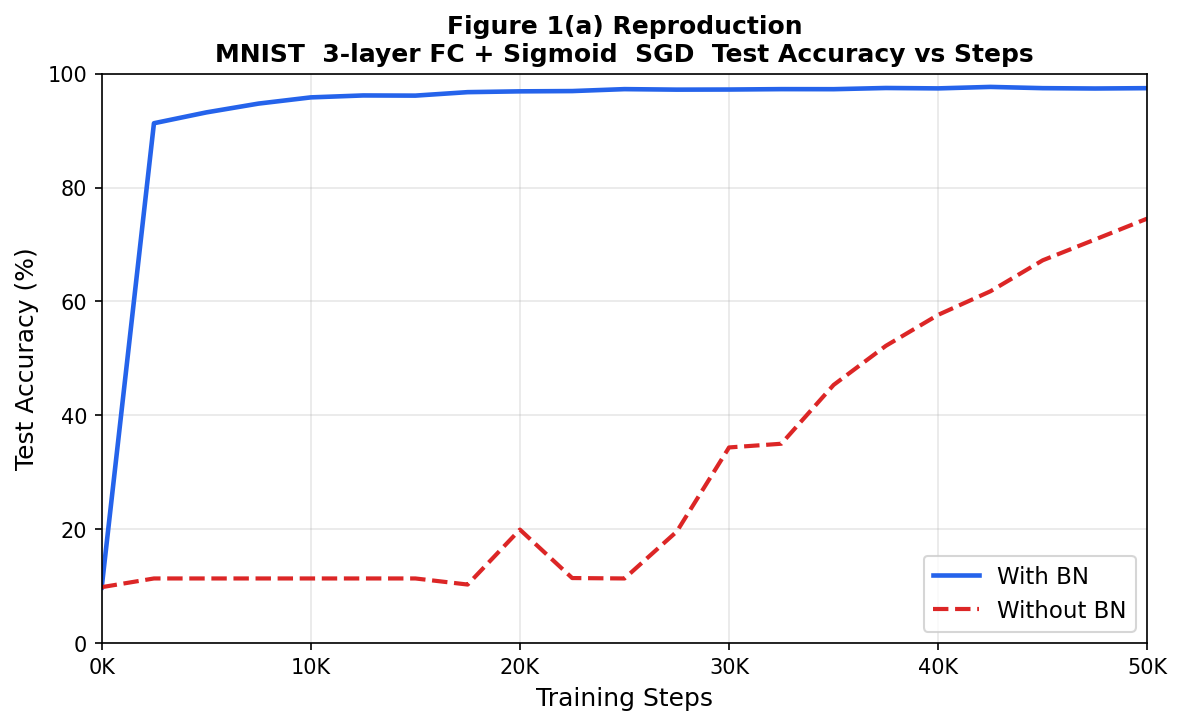
\includegraphics[width=0.72\linewidth]{exp1_figure1a_reproduction.png}
  \caption{Test accuracy vs.\ training steps on MNIST. Blue solid = With BN; red dashed =
  Without BN. The BN model converges in $\sim$5K steps while the non-BN model reaches
  $\sim$75\% at 50K steps. Reproduces Figure~1(a) of Ioffe \& Szegedy (2015).}
  \label{fig:exp1a}
\end{figure}

This represents a $>$20 percentage point improvement in final accuracy alongside a substantial
convergence speedup. The qualitative pattern closely matches Figure~1(a) of the original paper.
The mechanism is consistent with the paper's explanation: without BN, pre-activation values
drift into the saturated regime of the sigmoid, causing vanishing gradients. BN keeps these
values in the linear regime, enabling effective gradient flow throughout training.

\paragraph{Part B: Validation: Effect of Hidden Layer Width.}
To verify that BN's benefit is not specific to the paper's choice of 100 hidden units, we
sweep hidden widths across \{50, 100, 200\} units, holding all other hyperparameters constant.
Table~\ref{tab:exp1b} summarizes the final test accuracies after 50\,000 steps, and
Figure~\ref{fig:exp1b} shows the corresponding bar chart.

\begin{table}[h]
  \caption{Final test accuracy (\%) at 50K steps across hidden layer widths (MNIST).}
  \label{tab:exp1b}
  \centering
  \begin{tabular}{cccc}
    \toprule
    Hidden Units & Without BN (\%) & With BN (\%) & Improvement (pp) \\
    \midrule
    50  & 73.2 & 97.3 & +24.1 \\
    100 & 79.6 & 97.5 & +17.9 \\
    200 & 83.7 & 97.8 & +14.1 \\
    \bottomrule
  \end{tabular}
\end{table}

\begin{figure}[h]
  \centering
  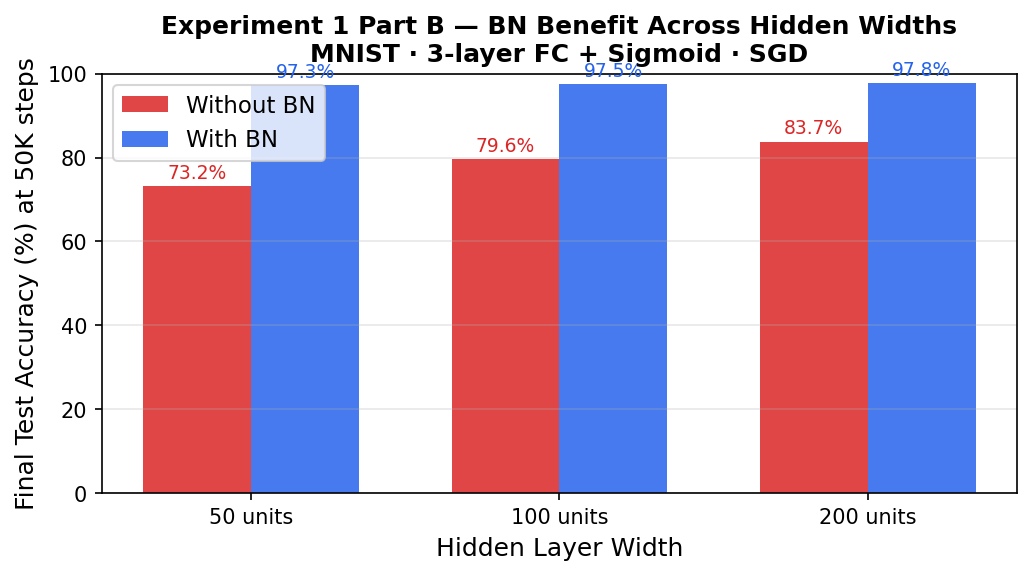
\includegraphics[width=0.65\linewidth]{exp1b_width_ablation.png}
  \caption{Final test accuracy across hidden layer widths. BN (blue) maintains $\sim$97\%
  at all widths; non-BN (red) improves with width but consistently lags by 14--24 pp.}
  \label{fig:exp1b}
\end{figure}

BN consistently outperforms the non-BN baseline at all widths. While wider networks slightly
improve the non-BN model (more parameters reduce the sigmoid-saturation bottleneck), the gap
remains substantial in all cases, demonstrating that BN's benefit is robust to network size.

\subsection{Experiment 2: CIFAR-10 CNN: Learning Rate Sensitivity}

\paragraph{Setup.}
We implement a 6-convolution-layer CNN with two convolutional blocks (3$\to$32$\to$32 and
32$\to$64$\to$64 channels), max pooling, global average pooling, and a fully connected output
layer. BN is applied after each convolution and before the ReLU activation
(\texttt{Conv $\to$ BN $\to$ ReLU}), following Section~3.2 of the paper. The non-BN and BN
models are architecturally identical except for the presence of \texttt{BatchNorm2d} layers.
Training uses SGD with momentum 0.9 for 15 epochs on CIFAR-10. We sweep three learning rates:
\{0.001, 0.01, 0.1\}. SGD with momentum is deliberately chosen because its non-adaptive update
rule makes divergence at high learning rates clearly visible, unlike Adam, which masks
instability through adaptive step sizes.

\paragraph{Part A: Reproduction of LR Sensitivity (Section~3.3).}
Table~\ref{tab:exp2a} summarizes the final test accuracies, and Figure~\ref{fig:exp2a} shows
training loss, training accuracy, and test accuracy over epochs for all six (LR, BN)
combinations.

\begin{table}[h]
  \caption{Final test accuracy (\%) after 15 epochs on CIFAR-10 across learning rates.}
  \label{tab:exp2a}
  \centering
  \begin{tabular}{lccc}
    \toprule
    Learning Rate & Without BN (\%) & With BN (\%) & Outcome \\
    \midrule
    0.001 & $\sim$30   & $\sim$75--80 & BN converges faster and higher \\
    0.01  & $\sim$70--75 & $\sim$78--80 & Both train; BN more stable \\
    0.1   & $\sim$10 (diverges) & $\sim$80 & Non-BN fails; BN trains stably \\
    \bottomrule
  \end{tabular}
\end{table}

\begin{figure}[h]
  \centering
  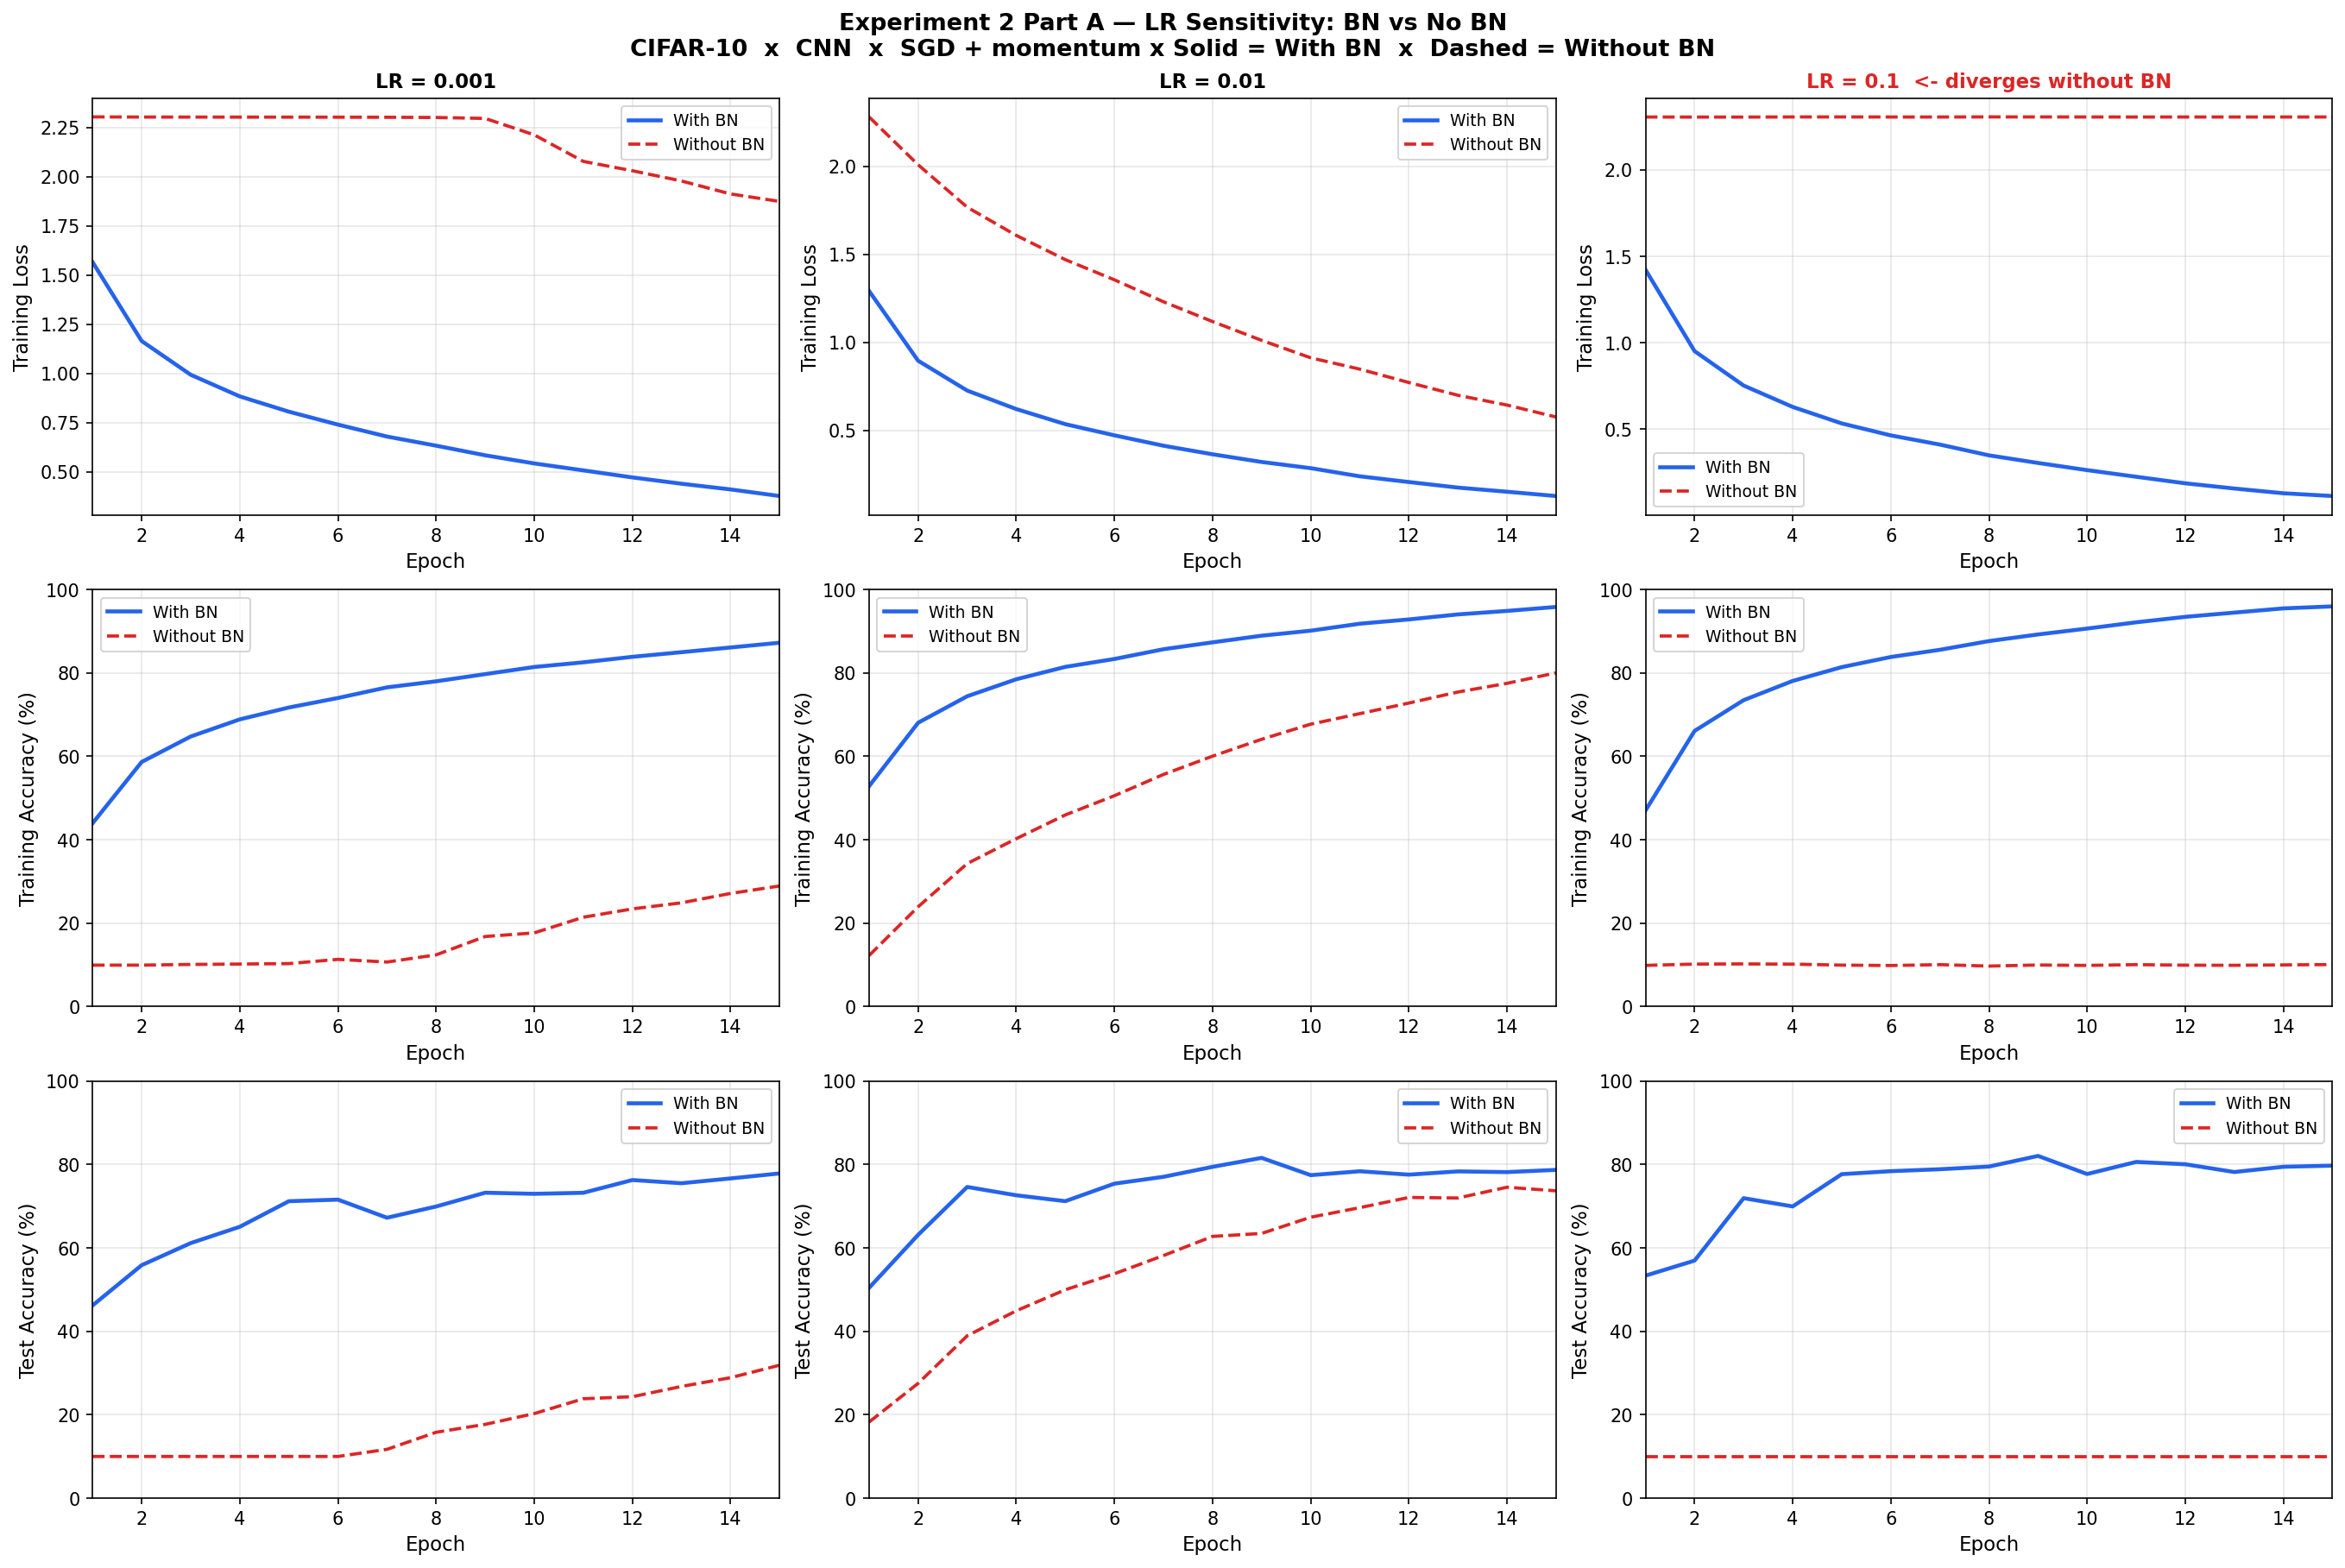
\includegraphics[width=\linewidth]{exp2a_lr_sensitivity.png}
  \caption{Training loss (top), training accuracy (middle), and test accuracy (bottom) over
  15 epochs on CIFAR-10, for LR $\in$ \{0.001, 0.01, 0.1\} (columns). Blue solid = With BN;
  red dashed = Without BN. At LR = 0.1, the non-BN model diverges immediately while the BN
  model trains stably to $\sim$80\%.}
  \label{fig:exp2a}
\end{figure}

The most striking result is at LR = 0.1: the non-BN model fails to learn at all, remaining
near chance ($\sim$10\%), while the BN model trains stably and reaches approximately 80\% test
accuracy. This directly reproduces the paper's central claim from Section~3.3: BN makes
training resilient to high learning rates because its scale-invariance property decouples
gradient magnitudes from parameter scale. The non-BN model at LR = 0.1 exhibits classic
gradient explosion: loss becomes NaN in the first few epochs and accuracy stays at chance
throughout.

\paragraph{Part B: Validation: Optimizer Ablation.}
To probe whether the instability at LR = 0.1 is SGD-specific or a general property that BN
addresses, we replace SGD+momentum with Adam at the same learning rate. Adam uses adaptive
per-parameter learning rates, which inherently dampen large gradient updates.

\begin{figure}[h]
  \centering
  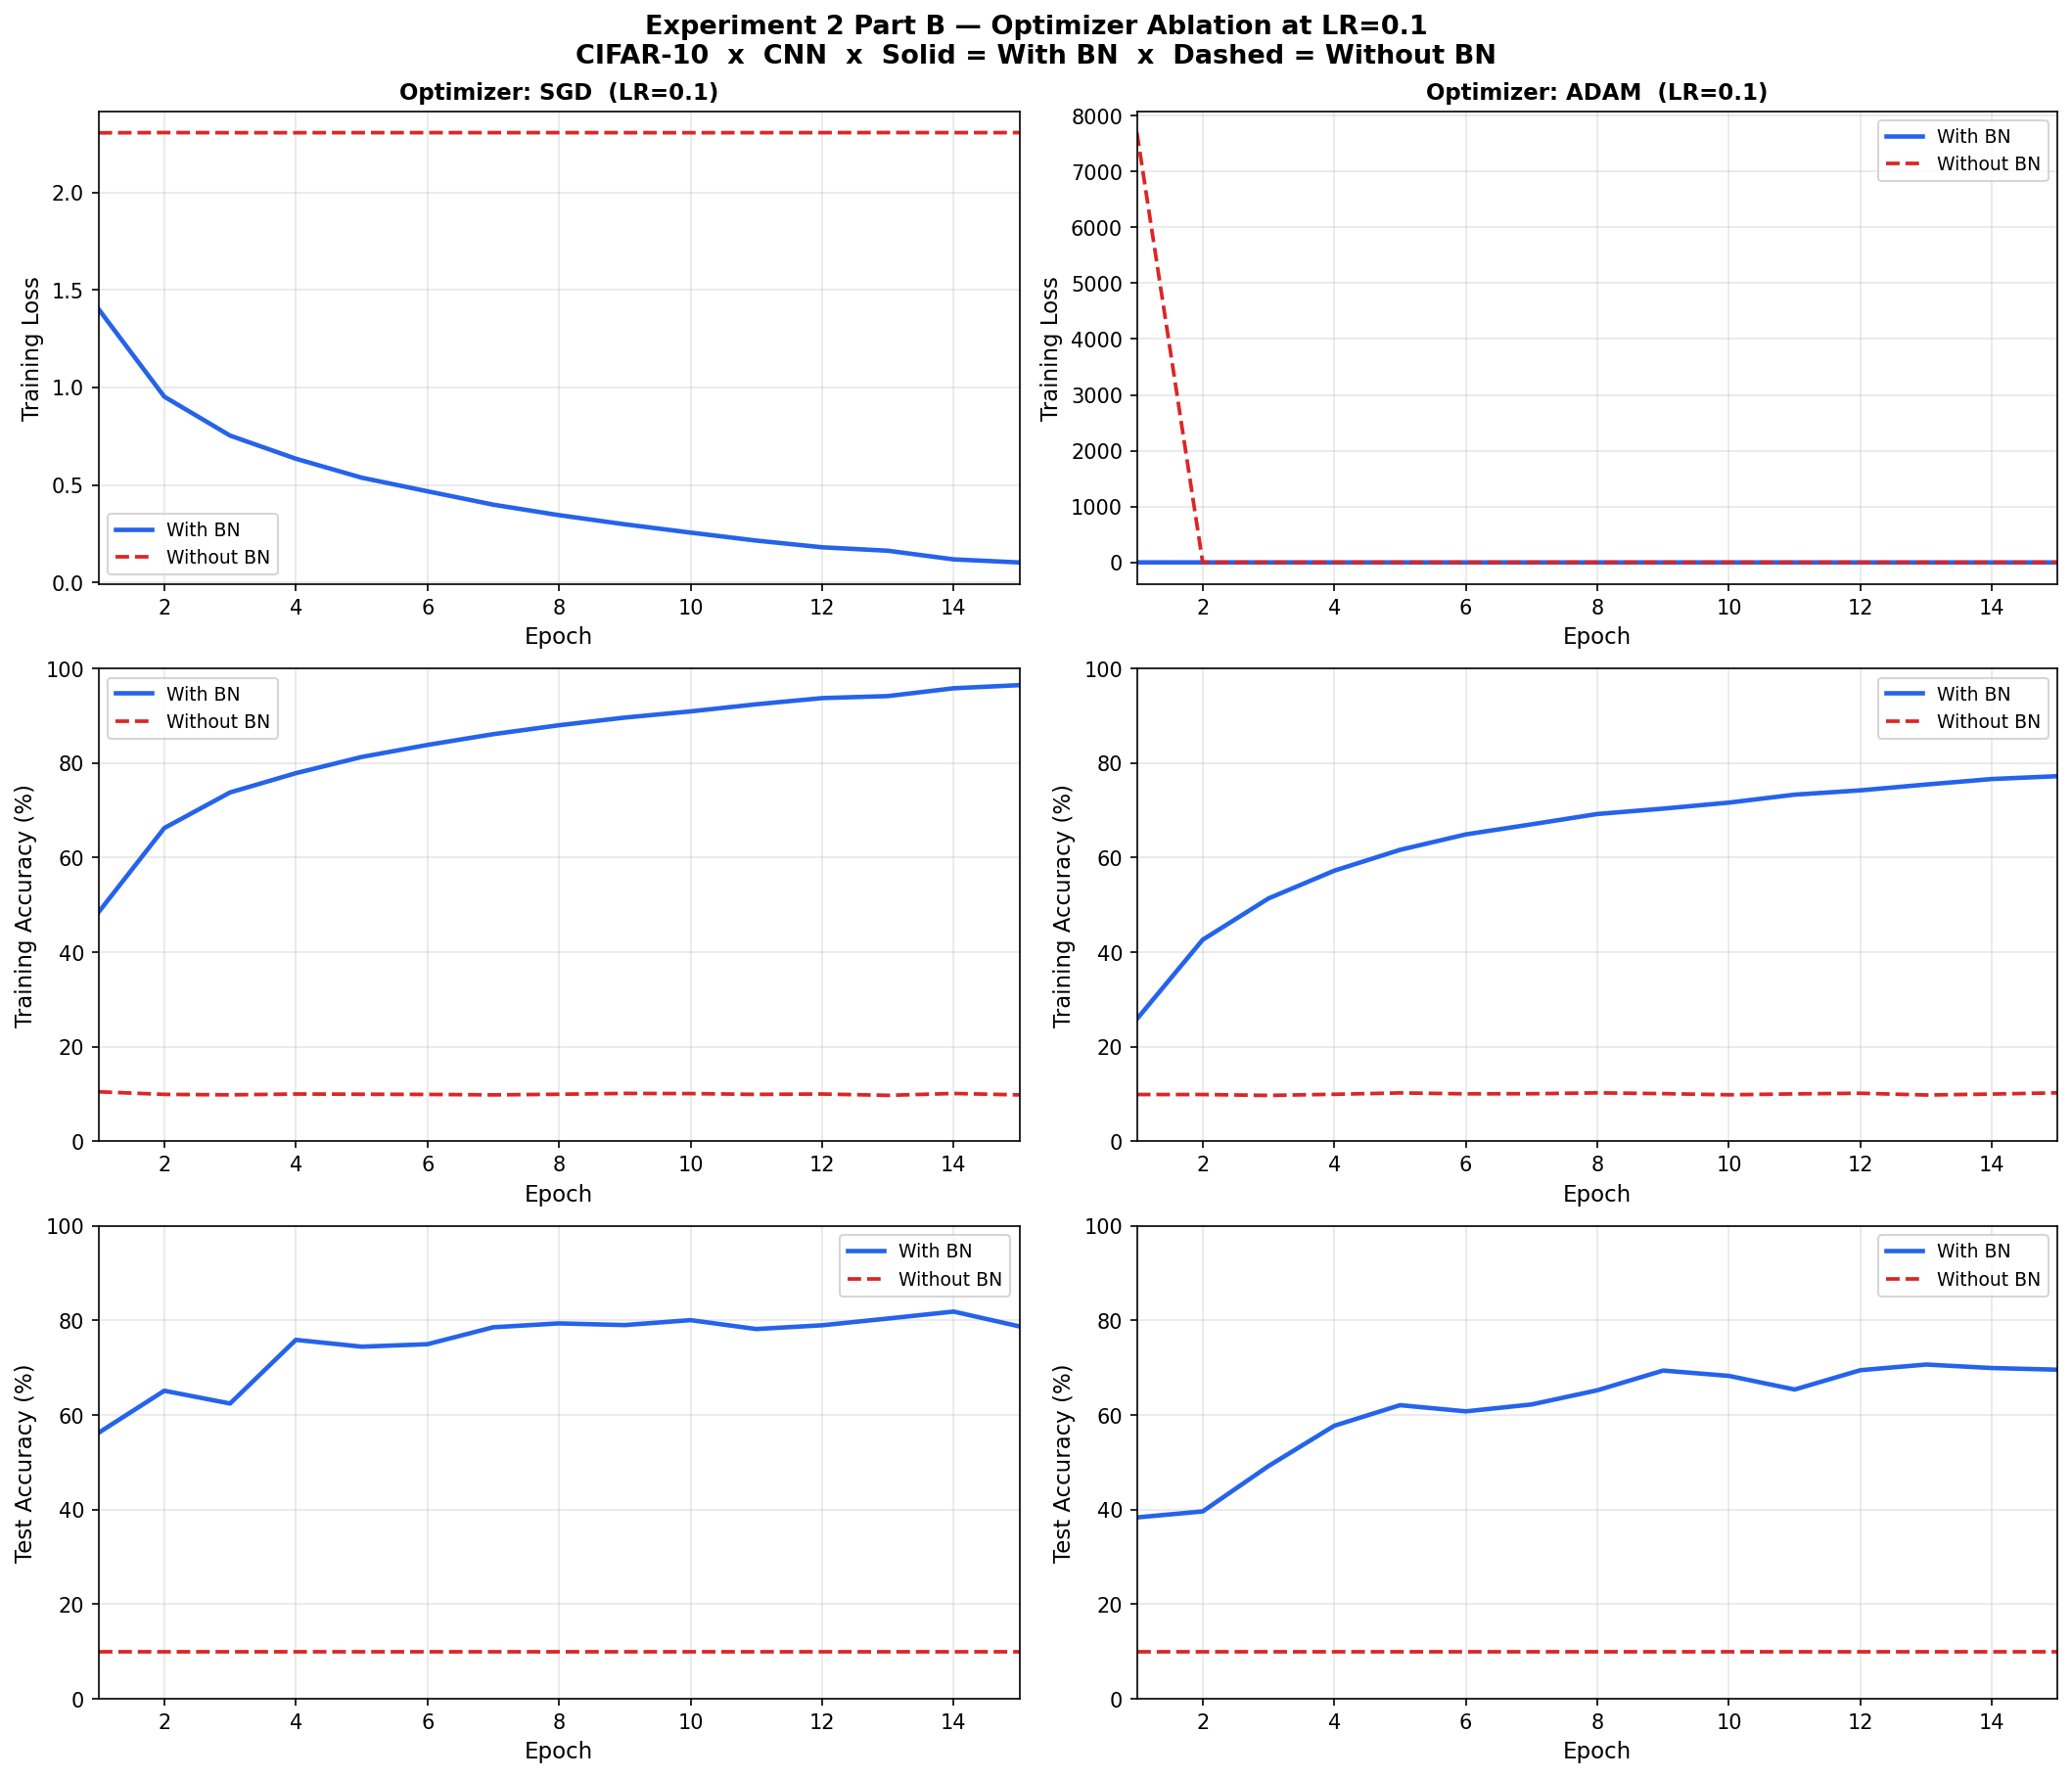
\includegraphics[width=0.85\linewidth]{exp2b_optimizer_ablation.png}
  \caption{Optimizer ablation at LR = 0.1 on CIFAR-10. Left column = SGD+momentum; right
  column = Adam. Both optimizers without BN (red dashed) diverge; both with BN (blue solid)
  converge. SGD+BN reaches $\sim$80\%; Adam+BN reaches $\sim$70\%.}
  \label{fig:exp2b}
\end{figure}

Surprisingly, Adam without BN also becomes numerically unstable at LR = 0.1. With BN, Adam
converges stably to approximately 70\% test accuracy, somewhat below the SGD+BN result, likely
because Adam's adaptive updates interact differently with the already-normalized activations.
This result reinforces that BN's stabilization benefit is not optimizer-specific, and that
LR = 0.1 is genuinely pathological for this architecture regardless of optimizer.


%% =============================================================================
\section{Comparison with Related Normalization Methods}
%% =============================================================================

Batch Normalization was one of the first normalization techniques to be integrated directly
into the model architecture, but it is far from the only one. In this section, we compare BN
against two related approaches that address similar problems from different angles: Root Mean
Square Layer Normalization (RMSNorm)~\cite{zhang2019rmsnorm} and Z-Score input
standardization~\cite{alfaiz2018zscore}. Understanding where BN sits relative to these methods
helps clarify both what makes it powerful and where its limitations lie.

\subsection{Root Mean Square Layer Normalization (RMSNorm)}

Zhang and Sennrich~\cite{zhang2019rmsnorm} propose RMSNorm as a simplified and more
computationally efficient alternative to Layer Normalization (LayerNorm). While BN normalizes
across the batch dimension using mini-batch statistics, LayerNorm normalizes across the feature
dimension within a single training example, making it well suited for sequence models like
RNNs and Transformers where batch-based statistics are impractical. RMSNorm takes this one
step further by dropping the mean subtraction (re-centering) entirely and normalizing only
by the root mean square of the activations:
\begin{equation}
  \bar{a}_i = \frac{a_i}{\mathrm{RMS}(\mathbf{a})}\, g_i, \quad
  \text{where} \quad \mathrm{RMS}(\mathbf{a}) = \sqrt{\frac{1}{n}\sum_{i=1}^{n} a_i^2}
\end{equation}
The core argument is that re-scaling invariance, not re-centering invariance, is the property
that actually matters for stable training. By removing the mean subtraction, RMSNorm is faster
to compute and has a simpler backward pass, while still giving the gradient stability benefits
that LayerNorm provides.

This is actually an interesting point to think about in the context of our BN experiments.
BN normalizes both the mean and variance of activations, but the Santurkar et al.
argument~\cite{santurkar2018does} we discussed earlier suggests that it is the smoothing of
the loss landscape, rather than the explicit mean centering, that drives the improvement.
RMSNorm provides some indirect evidence for this: dropping re-centering entirely has little
effect on model quality. Zhang and Sennrich show that across machine translation, reading
comprehension, image-caption retrieval, and image classification tasks, RMSNorm matches
LayerNorm in final accuracy while running 7\% to 64\% faster depending on the architecture
and framework.

The key practical difference between BN and RMSNorm comes down to what dimension is being
normalized and when. BN normalizes across the batch at training time, which means its
statistics become noisy at small batch sizes and requires separate handling at inference time.
RMSNorm normalizes within a single example at each step, which makes it batch-size independent
and equally valid at training and inference. This is why RMSNorm (and LayerNorm more broadly)
has largely replaced BN in modern Transformer architectures, where sequences have variable
length and batching is more constrained. That said, BN still tends to outperform LayerNorm and
RMSNorm in image classification settings. Zhang and Sennrich's own CIFAR-10 experiments show
that BatchNorm achieves 8.25\% test error compared to RMSNorm's 8.83\% and LayerNorm's
10.49\% on their ConvPool-CNN-C model, which is consistent with our own observation that BN
provides very strong benefits for CNN training on image data.

\subsection{Z-Score Input Standardization}

Al-Faiz et al.~\cite{alfaiz2018zscore} study a conceptually simpler form of normalization:
applying Z-score standardization to the network's \emph{input} data before training begins,
rather than normalizing internal activations during training. The Z-score transform is:
\begin{equation}
  z_{ij} = \frac{a_{ij} - \mu}{\alpha}
\end{equation}
where $\mu$ is the column mean and $\alpha$ is the column standard deviation. This is a static,
preprocessing step applied once before any training occurs. The paper studies this in the
context of a backpropagation network trained on binary data extracted from DNA gel
electrophoresis images, and compares Z-score against several other standardization methods
including Manhattan normalization, vector normalization, and bipolar transformation.

Their results show that Z-score standardization significantly reduces the number of training
epochs needed for convergence compared to using raw binary inputs, and outperforms the other
standardization methods in terms of final convergence speed. They also find that binary inputs
without any preprocessing are a serious problem: the zero values in the input effectively kill
gradient flow through the corresponding weights, which is very similar in spirit to the
vanishing gradient problem BN is designed to address in the hidden layers.

Comparing this to BN reveals both a conceptual connection and a fundamental difference.
The conceptual connection is that both methods are trying to improve gradient flow by keeping
activations in a more numerically well-conditioned range. Fixed Z-score input normalization
can be thought of as applying BN's effect once, at the input layer only, using the global
dataset statistics rather than mini-batch statistics. The fundamental difference is that BN
is dynamic and applied at every layer throughout the network, while Z-score standardization
is static and only applied to the raw input. This means Z-score standardization does nothing
to address the internal covariate shift problem that accumulates through the hidden layers as
training progresses. The benefit it provides is essentially equivalent to just normalizing
the input features, which is a common preprocessing step in machine learning regardless of
whether BN is used. In fact, the paper's best-performing method (Z-score) reaches convergence
in around 102 epochs at a learning rate of 0.0005 on their specific task, while bipolar
transformation achieves 113 epochs, showing that the differences between standardization
methods at the input level are relatively modest compared to the massive gap we observed
between BN and no-BN in our hidden layer experiments.

\subsection{Summary Comparison}

Table~\ref{tab:comparison} summarizes the key differences between the three approaches across
several dimensions that matter in practice.

\begin{table}[h]
  \caption{Comparison of Batch Normalization, RMSNorm, and Z-Score Standardization.}
  \label{tab:comparison}
  \centering
  \begin{tabular}{lccc}
    \toprule
    Property & Batch Norm & RMSNorm & Z-Score Std. \\
    \midrule
    Where applied       & Hidden layers (all) & Hidden layers (all) & Input only \\
    When applied        & Each training step  & Each training step  & Once (preprocessing) \\
    Statistics used     & Mini-batch          & Per-example RMS     & Full dataset \\
    Re-centering        & Yes                 & No                  & Yes \\
    Re-scaling          & Yes                 & Yes                 & Yes \\
    Batch-size dependent & Yes                & No                  & No \\
    Learnable params    & Yes ($\gamma$, $\beta$) & Yes ($g$)       & No \\
    Train/inference gap & Yes                 & No                  & No \\
    Best suited for     & CNNs, image tasks   & RNNs, Transformers  & Input preprocessing \\
    \bottomrule
  \end{tabular}
\end{table}

Overall, the three methods occupy different niches. Z-score standardization is the simplest
and cheapest option but only helps at the input boundary, leaving internal covariate shift
unaddressed. BN is the most powerful option for feedforward and convolutional networks because
it actively stabilizes activation distributions at every layer throughout training, which is
exactly the problem our experiments demonstrate is severe without it. RMSNorm is essentially
a more efficient evolution of LayerNorm that is better suited to sequence models, and the
finding that dropping re-centering has little effect is a useful insight into why BN works as
well as it does even though it computes more than strictly necessary. Each method reflects
a different understanding of the same underlying problem: getting gradients to flow cleanly
through a deep network.


%% =============================================================================
\section{Critical Evaluation}
%% =============================================================================

\subsection{Discrepancies from the Original Paper}

Our results are qualitatively consistent with the original paper, but quantitative differences
exist. In Experiment~1, the paper's Figure~1(a) shows the non-BN model reaching roughly 70\%
at 50\,000 steps, while ours reaches approximately 75--80\%. This minor discrepancy likely
reflects differences in weight initialization. PyTorch's default Kaiming uniform
initialization may provide a better starting point than the ``small random Gaussian values''
mentioned in the paper (without a specified variance). Both our BN and non-BN numbers are
slightly higher, suggesting our setup is marginally more favorable overall; the qualitative
relationship between the two curves is preserved exactly.

In Experiment~2, the paper does not provide exact CNN-on-CIFAR-10 numbers; its LR sensitivity
analysis is described qualitatively and demonstrated primarily on Inception-scale networks.
Direct numerical comparison is therefore not possible, but the qualitative outcome of divergence
without BN at high LR, stability with BN precisely matches the paper's predictions.

\subsection{Limitations}

Our reproduction has several important limitations. First, both experiments use simplified
settings compared to the paper: MNIST and CIFAR-10 rather than ImageNet, and a small custom
CNN rather than Inception. The generalization of BN's benefits to large-scale settings is not
tested here.

Second, we report results from a single run per configuration, without error bars or confidence
intervals. Neural network training is stochastic, and single-run results can be noisy,
particularly for the non-BN model, whose training curves are sensitive to initialization.
Reporting results across multiple seeds would strengthen our conclusions.

Third, our Experiment~2 uses only 15 epochs, which may be insufficient for all models to
converge at the lower learning rates. A longer training run might reduce the performance gap
between BN and non-BN at LR = 0.001.

Fourth, the paper's theoretical explanation for BN's effectiveness has been contested.
Santurkar et al.~\cite{santurkar2018does} argue that BN's primary benefit is smoothing the
loss landscape rather than directly reducing ICS. Our experiments confirm BN's empirical
benefits but do not adjudicate between these mechanistic explanations.

\subsection{Broader Implications}

Batch Normalization has become a standard component of virtually all modern deep learning
architectures. Beyond the benefits demonstrated here, BN reduces sensitivity to initialization,
acts as a mild regularizer (the paper notes it can replace Dropout in some settings), and
enables the use of saturating nonlinearities like sigmoid in deep networks.

However, BN introduces its own complications. Its effectiveness depends on batch size. At very
small batch sizes, mini-batch statistics become noisy and BN can hurt performance, motivating
alternatives such as Layer Normalization, Group Normalization, and Instance Normalization. BN
also introduces a training-inference mismatch (batch statistics vs.\ population statistics)
that can cause issues when the training and deployment distributions differ significantly.


%% =============================================================================
\section{Individual Reflections}
%% =============================================================================

Each group member provides an independent reflection on what they learned from this project
and from other groups' presentations.

\paragraph{Nathan Krosel.}
The most important thing I learned from this project was understanding why BN is 
applied to the pre-activation $Wu$ rather than after the nonlinearity. Because $Wu$ 
tends to have a more symmetric near-Gaussian distribution before the sigmoid is 
applied, normalizing it keeps inputs in the linear regime where gradients are 
non-negligible, whereas normalizing after the activation would constrain a 
distribution that has already been squashed in a much less predictable way. It also 
made the bias cancellation make sense to me, since BN subtracts the mini-batch mean 
anyway, any learned bias just gets cancelled before it affects the output, so the 
$\beta$ parameter completely takes over that role. From other group presentations I 
found the Adam paper really interesting because seeing how it maintains running 
estimates of the first and second gradient moments to build adaptive per-parameter 
step sizes made me realize that Adam and BN are essentially attacking the same 
instability problem from two completely different directions, one through the 
optimizer and one through the architecture itself.

\paragraph{Hetang Mehta.}
From this project I learned a lot more about how normalization actually works under 
the hood rather than just knowing it as something you add to your model. Before this 
I kind of just used batch norm without really thinking about why it helped, but going 
through the math and seeing the scale invariance property made it click for me. 
Reproducing the experiments also showed me how much the choice of optimizer and 
learning rate actually matters, since we saw the model completely fail at high learning 
rates without BN. From other group presentations the superposition disentanglement 
paper was the most surprising to me because I had never considered that two models 
could learn identical features but arrange them across neurons so differently that 
standard alignment metrics would score them as dissimilar, which made me think about 
how much of what we measure in deep learning is actually an artifact of how we choose 
to measure it.

\paragraph{Maanas Saxena.}
What stood out to me the most from this project was the connection between batch 
normalization and the broader question of why deep networks are hard to train. Before 
this course I knew sigmoid was bad for deep networks but I never fully understood why, 
and seeing it completely fail in our experiment without BN while working fine with it 
made that concrete in a way that reading about it never did. I also found it genuinely 
surprising that dropping the re-centering step entirely, like RMSNorm does, barely 
hurts performance, which made me question how much of what BN does is actually 
necessary versus just convenient. From other groups I thought the Adam paper was 
really well presented because the idea of maintaining bias-corrected moment estimates 
to get stable adaptive learning rates is elegant, and seeing it explained clearly made 
me appreciate how much thought went into something that most people just use as a 
default without questioning.

\paragraph{Nathan Wong.}
From our project, the biggest thing I learned was that there was more to training a 
model than just selecting different architectures. I always assumed that once you had 
a good architecture, the training details were mostly secondary, but this project showed 
that things like normalization, learning rate, and optimizer choice can be the 
difference between a model that works and one that completely diverges and never 
learns anything. I also learned a lot from actually going through the implementation 
because there were small details in the paper, like removing biases before BN layers 
and using population statistics at inference, that you would easily miss if you were 
just reading at a high level. Out of all the other papers, the superposition disentanglement paper stood out to me because it showed that certain learned features line up across different models, even when those models are trained separately. This suggests that deep networks may be learning more consistent and universal patterns than it seems when you look only at individual neurons, and showed a very interesting look into how the models actually work.


%% =============================================================================
\section*{References}
%% =============================================================================

\begin{thebibliography}{9}

\bibitem{ioffe2015batch}
Ioffe, S.\ \& Szegedy, C.\ (2015).
Batch Normalization: Accelerating Deep Network Training by Reducing Internal Covariate Shift.
\textit{Proceedings of the 32nd International Conference on Machine Learning (ICML)},
JMLR: W\&CP volume 37.

\bibitem{santurkar2018does}
Santurkar, S., Tsipras, D., Ilyas, A.,\ \& Madry, A.\ (2018).
How Does Batch Normalization Help Optimization?
\textit{Advances in Neural Information Processing Systems 31 (NeurIPS)}.

\bibitem{zhang2019rmsnorm}
Zhang, B.\ \& Sennrich, R.\ (2019).
Root Mean Square Layer Normalization.
\textit{Advances in Neural Information Processing Systems 32 (NeurIPS 2019)}.
arXiv:1910.07467.

\bibitem{alfaiz2018zscore}
Al-Faiz, M.\ Z., Ibrahim, A.\ A.,\ \& Hadi, S.\ M.\ (2018).
The Effect of Z-Score Standardization on Binary Input Due the Speed of Learning in
Back-Propagation Neural Network.
\textit{Iraqi Journal of Information and Communications Technology}, Vol. 1, Issue 3.

\bibitem{lecun1998}
LeCun, Y., Bottou, L., Bengio, Y.,\ \& Haffner, P.\ (1998).
Gradient-based learning applied to document recognition.
\textit{Proceedings of the IEEE}, 86(11), 2278--2324.

\bibitem{krizhevsky2009}
Krizhevsky, A.\ (2009).
Learning Multiple Layers of Features from Tiny Images.
Technical Report, University of Toronto.

\bibitem{paszke2019pytorch}
Paszke, A.\ et al.\ (2019).
PyTorch: An Imperative Style, High-Performance Deep Learning Library.
\textit{Advances in Neural Information Processing Systems 32 (NeurIPS)}.

\end{thebibliography}


%% =============================================================================
\appendix
\section{Experimental Details}
%% =============================================================================

\paragraph{Hardware and runtime.}
All experiments were run on Apple Silicon (MPS backend) or CPU. Experiment~1 (two runs of
50\,000 steps, batch size 60) completes in approximately 15--20 minutes per run. Experiment~2
(six combinations of LR and BN $\times$ 15 epochs on CIFAR-10) completes in approximately
30--45 minutes total. No GPU cluster was used; all experiments are reproducible on a standard
laptop or Google Colab.

\paragraph{Hyperparameter summary.}

\begin{table}[h]
  \caption{Hyperparameters for all experiments.}
  \centering
  \begin{tabular}{lll}
    \toprule
    Parameter & Experiment 1 & Experiment 2 \\
    \midrule
    Dataset         & MNIST         & CIFAR-10 \\
    Batch size      & 60            & 64 \\
    Steps / Epochs  & 50\,000 steps & 15 epochs \\
    Optimizer       & SGD           & SGD + momentum 0.9 \\
    Learning rate   & 0.01          & \{0.001, 0.01, 0.1\} \\
    Hidden units    & 100 (+ ablation: 50, 200) & N/A \\
    BN placement    & FC $\to$ BN $\to$ Sigmoid & Conv $\to$ BN $\to$ ReLU \\
    Random seed     & 42            & 42 \\
    \bottomrule
  \end{tabular}
\end{table}


%% =============================================================================
\newpage
\section*{NeurIPS Paper Checklist}
%% =============================================================================

\begin{enumerate}

\item \textbf{Claims}
  \item[] Question: Do the main claims made in the abstract and introduction accurately reflect
  the paper's contributions and scope?
  \item[] Answer: \answerYes{}
  \item[] Justification: The abstract explicitly states that we reproduce two qualitative
  phenomena (convergence acceleration on MNIST and LR stability on CIFAR-10) in simplified
  settings, and our results confirm both claims. We do not overstate generalization to
  large-scale settings.

\item \textbf{Limitations}
  \item[] Question: Does the paper discuss the limitations of the work performed by the authors?
  \item[] Answer: \answerYes{}
  \item[] Justification: Section~5.2 discusses limitations including use of simplified datasets
  (MNIST/CIFAR-10 vs.\ ImageNet), single-run results without error bars, short training in
  Experiment~2, and the contested theoretical explanation for BN's effectiveness.

\item \textbf{Theory assumptions and proofs}
  \item[] Question: For each theoretical result, does the paper provide the full set of
  assumptions and a complete (and correct) proof?
  \item[] Answer: \answerNA{}
  \item[] Justification: This is a reproduction paper with no novel theoretical results. We
  present the BN algorithm and its key properties (scale invariance, backpropagation formulas)
  as described in the original paper.

\item \textbf{Experimental result reproducibility}
  \item[] Question: Does the paper fully disclose all the information needed to reproduce the
  main experimental results?
  \item[] Answer: \answerYes{}
  \item[] Justification: All hyperparameters, architectures, optimizers, datasets, and random
  seeds are fully specified in Section~3 and the Appendix. The accompanying code notebook
  (submitted with the report) implements all experiments end-to-end.

\item \textbf{Open access to data and code}
  \item[] Question: Does the paper provide open access to the data and code?
  \item[] Answer: \answerYes{}
  \item[] Justification: Code is submitted as a Jupyter notebook alongside this report. Both
  MNIST and CIFAR-10 are publicly available standard benchmarks downloaded automatically via
  \texttt{torchvision.datasets}.

\item \textbf{Experimental setting/details}
  \item[] Question: Does the paper specify all training and test details necessary to
  understand the results?
  \item[] Answer: \answerYes{}
  \item[] Justification: Section~3 and the Appendix table specify datasets, splits, batch
  sizes, optimizers, learning rates, number of steps/epochs, architectures, BN placement,
  and the random seed used for reproducibility.

\item \textbf{Experiment statistical significance}
  \item[] Question: Does the paper report error bars or other appropriate information about
  statistical significance?
  \item[] Answer: \answerNo{}
  \item[] Justification: Due to computational constraints (each experiment requires 15--20
  minutes per run), we report results from a single run per configuration. This is acknowledged
  as a limitation in Section~5.2. The qualitative phenomena we reproduce (convergence curves
  and divergence at high LR) are consistent and clear even without multiple runs.

\item \textbf{Experiments compute resources}
  \item[] Question: Does the paper provide sufficient information on compute resources?
  \item[] Answer: \answerYes{}
  \item[] Justification: The Appendix states that all experiments were run on Apple Silicon
  (MPS) or CPU, with estimated runtimes of 15--20 minutes for Experiment~1 and 30--45 minutes
  for Experiment~2. No specialized hardware was used.

\item \textbf{Code of ethics}
  \item[] Question: Does the research conform with the NeurIPS Code of Ethics?
  \item[] Answer: \answerYes{}
  \item[] Justification: This is a reproduction study using standard public benchmarks (MNIST,
  CIFAR-10). No data collection, human subjects, or potentially harmful applications are
  involved.

\item \textbf{Broader impacts}
  \item[] Question: Does the paper discuss both positive and negative societal impacts?
  \item[] Answer: \answerNA{}
  \item[] Justification: This is a reproduction of a foundational ML training technique using
  standard image classification benchmarks. There is no direct path to negative societal
  impact from this work; the technique itself is a general optimization aid with no specific
  harmful application.

\item \textbf{Safeguards}
  \item[] Question: Does the paper describe safeguards for responsible release of data or models?
  \item[] Answer: \answerNA{}
  \item[] Justification: We do not release new models, datasets, or systems. We use only
  publicly available datasets (MNIST, CIFAR-10) and train small classification models for
  educational purposes.

\item \textbf{Licenses for existing assets}
  \item[] Question: Are creators of assets properly credited with licenses mentioned?
  \item[] Answer: \answerYes{}
  \item[] Justification: The original BN paper (Ioffe \& Szegedy, 2015), RMSNorm
  (Zhang \& Sennrich, 2019), Z-score standardization (Al-Faiz et al., 2018), and
  PyTorch~\cite{paszke2019pytorch} are all cited. MNIST and CIFAR-10 are cited via their
  original papers~\cite{lecun1998,krizhevsky2009}. All datasets are freely available for
  research use.

\item \textbf{New assets}
  \item[] Question: Are new assets introduced in the paper well documented?
  \item[] Answer: \answerNA{}
  \item[] Justification: This paper does not introduce new datasets, models, or other releasable
  assets beyond the reproduction code, which is documented via inline comments throughout the
  notebook.

\item \textbf{Crowdsourcing and research with human subjects}
  \item[] Question: Does the paper include details of crowdsourcing or human subjects research?
  \item[] Answer: \answerNA{}
  \item[] Justification: No crowdsourcing or human subjects are involved in this work.

\item \textbf{Institutional review board (IRB) approvals}
  \item[] Question: Does the paper describe IRB approvals for human subjects research?
  \item[] Answer: \answerNA{}
  \item[] Justification: No human subjects research is conducted in this work.

\item \textbf{Declaration of LLM usage}
  \item[] Question: Does the paper describe usage of LLMs as a core component of the methods?
  \item[] Answer: \answerNA{}
  \item[] Justification: No LLMs are used as part of the core methodology. LLMs were used
  only for writing assistance and do not impact the experimental design, implementation, or
  results.

\end{enumerate}

\end{document}